\subsection{Architektura webu}
Pro lepší představu o funkci webu vám nyní vysvětlím, co všechno se stane, pokud stránku navštívíte.

Vše začne zadáním adresy \href{https://www.worldee.com}{worldee.com} do adresního řádku (1). Požadavek se odešle na náš Next.js server, kde si ho jako první převezme middleware. Ten zkontroluje a případně upraví cookies a hlavičky požadavku a do url přidá lokalizaci. Potom ho předá routeru, který podle url najde většinou již předkreslenou požadovanou stránku, přeloží ji a posílá zpátky do prohlížeče (2).

Pokud byla stránka předem předkreslená, uživatel už nyní může vidět všechny její prvky, ač jde zatím jen o vizuál postrádají jakoukoliv funkčnost. Pokud ne, stránka je prázdná. Prohlížeč musí spustit React (3), stránku inicializovat a podle odpovědi serveru vytvořit všechny kompozice a komponenty. Po prvním renderu začíná probíhat komunikace s naším PHP serverem (4) a získaná data jsou z JSONu převáděna na použitelný formát (5), kterým jsou plněny datové třídy. Stránka je nyní plně načtená, celý proces trval jednotky sekund. 

\begin{figure}[!h]
    \centering
    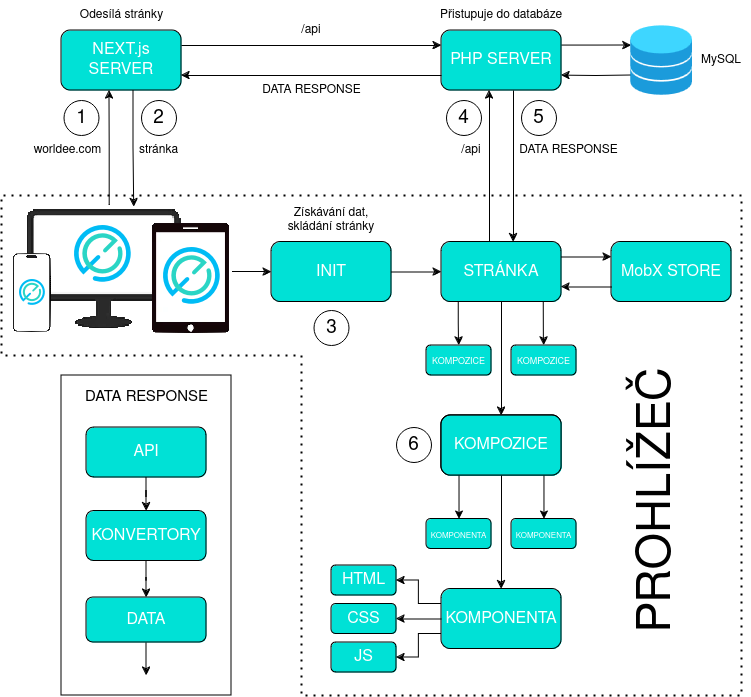
\includegraphics[width=1\linewidth]{obrazky/architektura.png}
    \caption{Diagram architektury webu}
\end{figure}
\clearpage

